\documentclass[a4paper, 14pt]{report}
\usepackage{cmap}
\usepackage[T2A]{fontenc}
\usepackage[top=3cm, bottom=3cm, left=3cm, right=3cm]{geometry}
\usepackage[utf8]{inputenc}
\usepackage[english,russian]{babel}
\usepackage{amsmath,amsfonts,amssymb,amsthm,mathtools}
\usepackage{hyperref}
\usepackage{graphicx}
\usepackage{wrapfig}
\usepackage{array}
\usepackage{hyperref}
\usepackage{booktabs}
\usepackage{array}
\usepackage{graphicx}
\usepackage{microtype}
\setlength{\extrarowheight}{4pt}


\begin{document}
\begin{titlepage}

\linespread{1.5}
\begin{center}

\textbf{Министерство науки и высшего образования Российской Федерации
Федеральное государственное автономное образовательное учреждение высшего образования\\ {\large КАЗАНСКИЙ (ПРИВОЛЖСКИЙ) ФЕДЕРАЛЬНЫЙ УНИВЕРСИТЕТ}}


\vspace{1cm}

\vspace*{\fill}

\textbf{{\LARGE \textbf{СЕМЕСТРОВАЯ РАБОТА}}\\
по дисциплине «Алгоритмы и анализ сложности»\\{\tiny {\large {\tiny }}}
«Экспериментальный анализ различных методов сортировки»}


\vspace{1.5cm}

\begin{flushleft}
    \textbf{\large Обучающийся: Величко Кирилл Андреевич гр. 09-041}\\
    \textbf{\large Руководитель: к.ф.-м.н., доцент КСАИТ, А. В. Васильев}
\end{flushleft}


\vspace*{\fill}
\textbf{\large Казань - 2023}

\vfill

\end{center}

\end{titlepage}

\tableofcontents
\section{Введение}
Цель работы: реализовать различные алгоритмы сортировки, провести замеры производительности реализованных алгоритмов
 на различных типах данных, объемах и распределениях.
 
Используемые технологии: C++ 20 стандарт.
 
В ходе проведения зачетной работы были реализованы следующие алгоритмы: сортировка пузырьком, сортировка вставкой, сортировка выбором, сортировка Шелла,
сортировка Кучей, рекурсивная и нерекурсивная реализация сортировки слиянием, рекурсивная и нерекурсивная реализация Быстрой сортировки по схеме Хоара,
реализована рекурсивная и нерекурсивная реализация поразрядной сортировки, на основе полученных данных реализована гибридная сортировка.

Также, была создана обертка над стандартной сортировкой std::sort. 


\section{Методика проведения эксперемента}
Эксперимент проводится следующим образом - были реализованы описанные во введении алгоритмы сортировок, написаны генераторы входных последовательностей,
если быть точнее - реализованы шаблонные функции высшего порядка, которые в зависимости от заданного типа распределения и типа генерируемых данных 
возвращают лямбда-выражение, принимающее непосредственно размеры входной последовательности, а также некоторые параметры вероятностных распределений.
Реализована генерация цифр, чисел, строк, а объектов типа Дата. Также были реализованы следующие распределения: равномерное распределение,
нормальное распределение, а также 2 типа частично отсортированных входных последовательностей, у которых есть в наличии некоторый интервал данных,
на котором находятся неупорядоченные данные, полученные за счет обмена значениями либо присвоения случайного значения в зависимости от типа генерации.

Далее, для различных сортировок, распределений, объемов и типов данных произведены замеры затраченного на сортировку времени, которые отображены на соответствующих графиках. 

Исходя из полученных результатов написана гибридная сортировка, адаптированная под работу с различными типами входных данных.
\section{Ход работы}
Для начала, были реализованы различные типы сортировок. Все сортировки, кроме поразрядной сортировки имеют единообразных интерфейс: итератор на начало последовательности, итератор на конец последовательности, некоторый компаратор. В случае поразрядной сортировки вместо компаратора передается функция отображения объекта на беззнаковое целочисленное значение. Реализации большинства сортировок абсолютно стандартны, в то время как в случае поразрядной и быстрой сортировки есть нюансы, по моему мнению заслуживающие упоминания.

Начну с быстрой сортировки. Большинство схем, описанных в интернете, подразумевают отсутствие повторяющихся значений, либо же работают исключительно с численными типами данных. Быстрая сортировка, основанная на стандартной схеме Хоара, как раз таки работает исключительно с числовыми значениями, т.к.
для осуществления сортировки ей необходим пивот, основанный на среднем значении от начала и конца входной последовательности. В случае несоблюдения данного условия, по стандартной схеме Хаора возможно переполнение стека вызовов. Также, при неудачной последовательности при иначе выбранном пивоте возможен выход за границы массива при итерации по нему. Для решения данной проблемы, пивот создается из итератора начала и служит ограничителем для декрементирующего итератора. В этой ситуации проблему представляет инкрементирующий итератор, что решается за счет проверки на соответствие итератора итератору конца последовательности.

Теперь рассмотрим особенности реализации поразрядной сортировки. Большинство примеров реализуют поразрядную сортировку по базе 10, но это является плохим решением, т.к. в этом случае приходится выполнять дорогую операцию деления на десять, что при больших объемах данных представляет из себя проблему. Вместо этого я выбрал базу 256, т.к. она полнотью соответствует отдельному байту объекта, что позволяет не выполнять дорогие операции деления, а просто представить полученное из функции отображения число как char*, и на каждой итерации обращаться непосредственно к соответсвующему байту. Также, важно отметить, что на разных платформах у нас может быть разный порядок байт, что также учитывается при выполнении сортировки. Сортировка осуществляется в порядке от младшего байта к старшему. Более того, попытка реализовать данный алгоритм с использованием итераторов приводит к довольно низкой производительности, не оправдывающей данную реализацию. Вместо этого, мы будем копировать байтовые последовательности с помощью std::memcpy, что значительно повысит производительность данного алгоритма сортировки, что будет видно в дальнейшем на графиках. В качестве сравнения, также были оставлены медленные реализации поразрядной сортировки.

Перейдем непосредственно к измерениям. Для всех полученных результатов проводились замеры 10 раз, и из этих результатов высчитывалась средняя величина. Также, во время замера производительности
постарался максимально освободить ресурсы ЦП.

Результаты всех замеров представлены в микросекундах.

Для начала, посмотрим, как поведут себя различные сортировки на относительно небольшой последовательности строк из 5000 строк. Строки частично отсортированы

\begin{figure}[h]
	
	\centering
	
	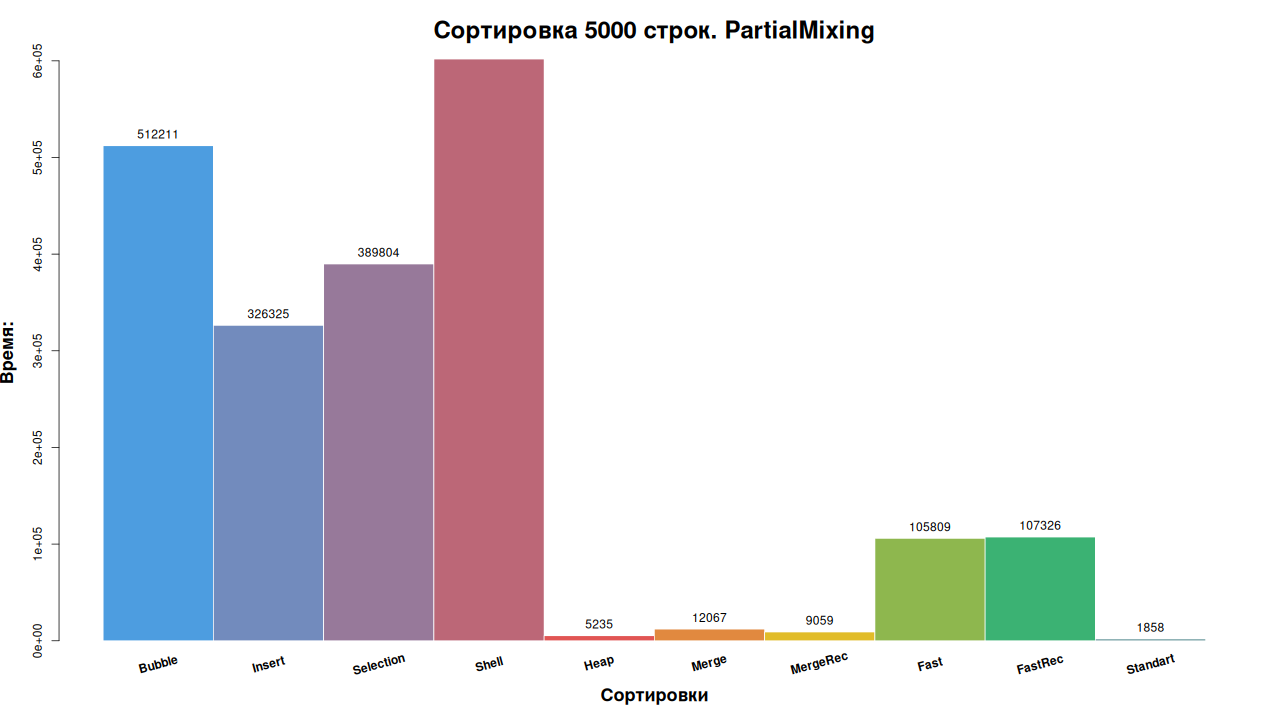
\includegraphics[width=0.8\linewidth]{./images/small_str.png}
	
	
	\label{fig:mpr}
	
\end{figure}


Как можно увидеть, на графике поразрядная сортировка остутствует. Она будет оценена отдельно.
Из графика становится очевидно, что наименьшей эффективностью обладают простейшие алгоритмы сортировки со сложностью ${n^2}$. Наиболее эффективно себя показала встроенная в язык сортировка, которая согласно документации является реализацией алгоритма IntroSort.

Рассмотрим больший объем данных, отбросив при этом неэффективные методы сортировки.

\begin{figure}[h]
	
	\centering
	
	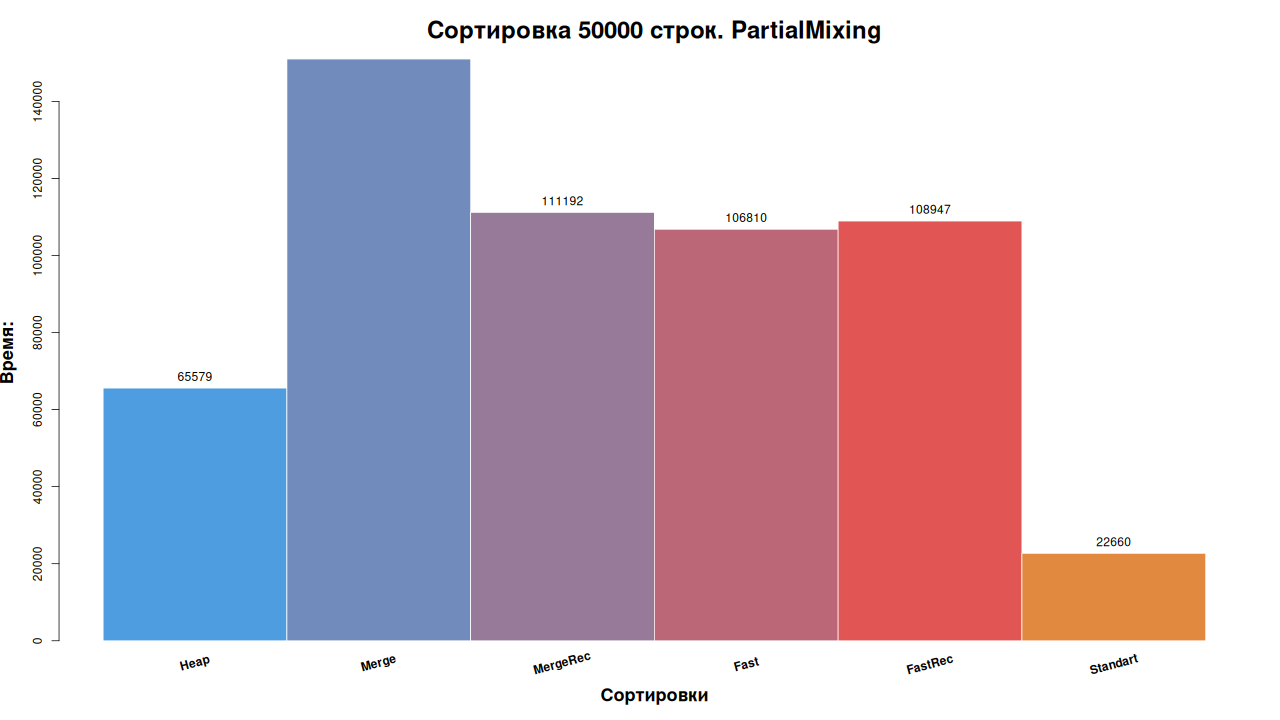
\includegraphics[width=0.8\linewidth]{./images/big_str.png}
	
	
	\label{fig:mpr}
	
\end{figure}

Как можно увидеть, большинство сортировок находится на примерно одинаковом уровне, из общей картины выбивается лишь стандартная сортировка и нерекурсивная сортировка слиянием. Более низкие результаты данного вида сортировки можно обусловить тем, что в процессе сортировки я использую изначальный буфер данных, практически не создавая новые. Это экономит память, но уменьшает произодительность. Также, из общей картины своей высокой производительностью выбивается сортировка кучей. Изучим ее более подробно.


\begin{figure}[h]
	
	\centering
	
	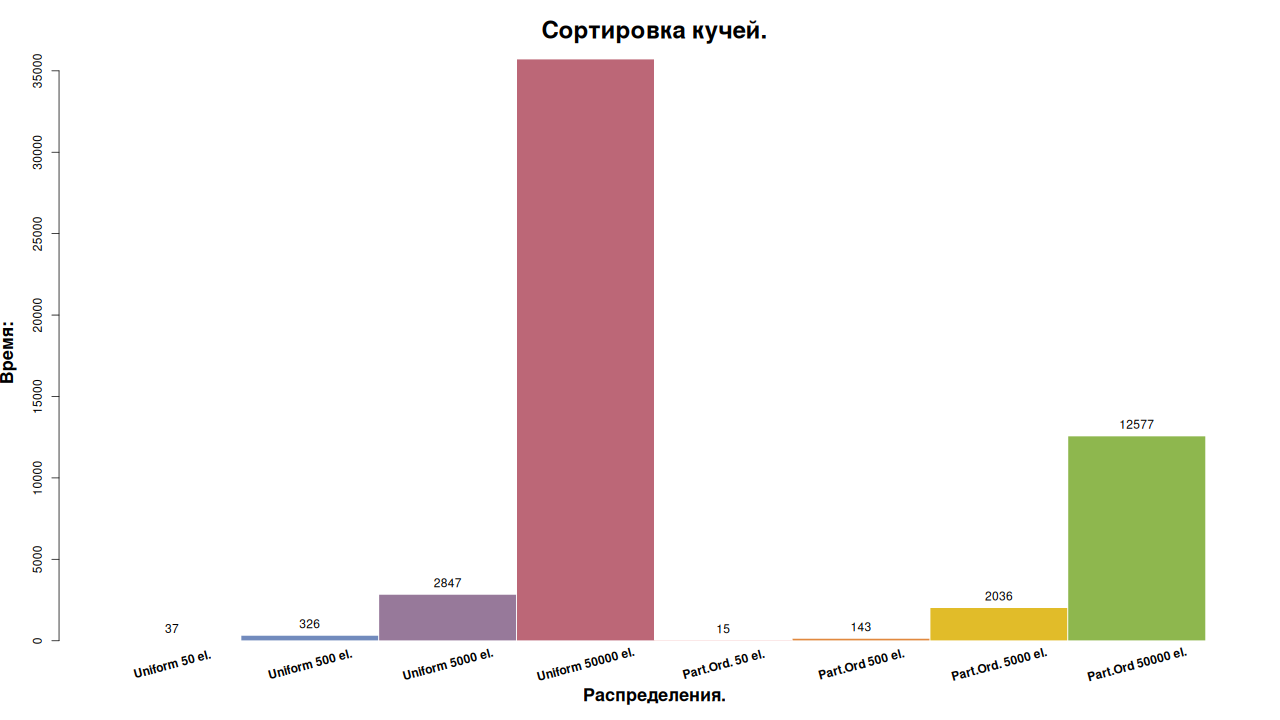
\includegraphics[width=0.8\linewidth]{./images/digit_heap.png}
	
	
	\label{fig:mpr}
	
На графике сравнивается произодительность сортировки кучей на частично отсортированной против равномерно распределенной последовательности. Как можно видеть из графика, сортировка кучей способна более эффективно обрабатывать последовательности с уже имеющейся упорядоченностью. Это свойство связано с тем, что, если параметры компаратора уже совпадают с параметрами кучи и прежде всего в кучу будут добавляться старшие элементы, то дальнейшее добавление элементов в кучу в среднем более эффективно, т.к. не придется протаскивать добавляемые элементы через все "дерево". В то же время, сортировка слиянием и быстрая сортировка подобными достоинствами не обладают.

В качестве проверки, стоит проверить результаты остальных алгоритмов и изучить, как соотносятся их результаты на случайных и частично отсортированных данных.
	
\end{figure}

\section{Заключение}
В случае работы с большими объемами данных, возникает опасность возникновения переполнения стека. Есть несколько способов решить данную проблему. Во-первых, очевидно, действительно большие объекты следует располагать в куче. Хоть лишние разыменования указателя и замедляет выполнение программы, в данной ситуации это является необходимостью. Во-вторых, зная размер объекта и их количество, можно установить лимит, при превышении которого массив данных тем или иным способом располагается на жестком диске, и уже к этим данным применяются алгоритмы внешней сортировки, то есть, данные будут сортироваться поблочно. Примером подобного алгоритма является внешняя сортировка слиянием.


1)При анализе принципа работы поразрядной сортировки, становится очевидно, в чем отличие данного вида сортировки от стандартных видов. Как видно из полученного программного кода, в то время как в более классических сортировках для непосредственной сортировки используются те или иные виды компараторов, для поразрядной сортировки необходимо построить функцию отображения объекта данного типа в некоторое число, желательно беззнаковое. И тут появляются 2 проблемы: во-первых, не для всех типов данных данную функцию отображения легко построить. Например, если мы сортируем строки в лексиграфическом порядке, то написание подобного компаратора не является проблемой. В то же время, для поразрядной сортировки это представляет некоторую трудность. Даже если мы рассмотрим строку, как некоторое число с разрядностью 256, то для строк разной длины подобная сортировка работать не будет, если мы будем идти от младшего байта к старшему. Если же идти от старшего байта к младшему, то данная проблема решается, но к подобному решению нужно еще прийти, а также интерфейс сортировки должен поддерживать подобную функцию. Во-вторых, проблемой также может являться сложность преобразования отдельных типов в число с точки зрения технической реализации. Эффективнее всего сравнивать разряды как раз-таки по основанию 256, т.к. тогда вместо медленных операций деления можно обращаться напрямую к интересующему нас байту. И тут возникают некоторые технические трудности. Например, в языке программирования Python числа имеют смешанный байтовый порядок, а нам для нормальной работы поразрядной сортировки нужен либо BigEndian, либо LittleEndian, из-за чего длинное число придется копировать в буфер с изменением порядка байт. В то время как классическая операция сравнения чисел справляется с этой задачей намного лучше. Таким образом, для сложных составных объектов поразрядная сортировка может иметь более низкую эффективность в связи довольно затратными операциями по отображению в число, особенно при относительно «небольших» размерах данных.
Исходя из данных рассуждений, становится понятно, что лучше всего сортировать с помощью поразрядной сортировки типы, легко представляемые в виде числа. Например, мы работаем в банке и храним данные клиентов. История каждого отдельного клиента может содержать такие параметры, как: текущая задолженность, сумма на каком-либо конкретном счете, и т.д. Соответственно, для подобных данных легко делать различные виды отображений, а большие объемы данных делают данную сортировку вполне оправданной. Единственное ограничение – превышение некоторого лимита допустимого размера для хранения в оперативной памяти. В этом случае, следует применить внешние сортировки.


2)Во-первых, стандартная сортировка имеет сложность n * logn, так что сортировки по типу цифровой и поразрядной на больших объемах данных ее точно обгонят, сложность заключается именно что в интеграции подобных сортировок с вашими данными. Во-вторых, стандартная сортировка подобрана так, чтобы в среднем показывать наиболее удовлетворительный результат на различных распределениях и размерах. На каком-либо конкретном распределении грамотно подобранная сортировка скорее всего обгонит стандартную. Однако, стоит отметить, что стандартная сортировка std::sort в C++ реализована как introsort, в сортировке используется быстрая сортировка, параметр глубины которой изначально определяется с помощью функции взятия быстрого логарифма по степени 2. В случае превышения глубины, используется partialsort. Std::sort написан очень качественно и обогнать его будет весьма затруднительно.

3)Простые методы сортировки имеет смысл использовать на относительно небольших размерах данных, либо же там, где высокая производительность не так критична. Ну и конечно, в подобных ситуациях имеет смысл использовать не простые сортировки, а стандартную сортировку, встроенную в язык.
4)На сортировку накладывает требования тип продукта, который мы разрабатываем. В первую очередь, ограничиваются требования к физическому способу хранения данных. Если мы разрабатываем СУБД, то нас интересуют алгоритмы внешних сортировок, позволяющие эффективно сортировать данные, лежащие в ПЗУ. Если же подобных требований нет, то лучше всего использовать наиболее универсальную сортировку, по типу быстрой сортировки или сортировки с помощью кучи. Но, конечно же, наиболее лучшим решением будет просто использовать стандартную сортировку.

\section{Приложение 1. Программный код}




\end{document}